\subsection{Magic Box}
\label{ch:prot_magicbox}
\begin{figure}[ht]
\centering
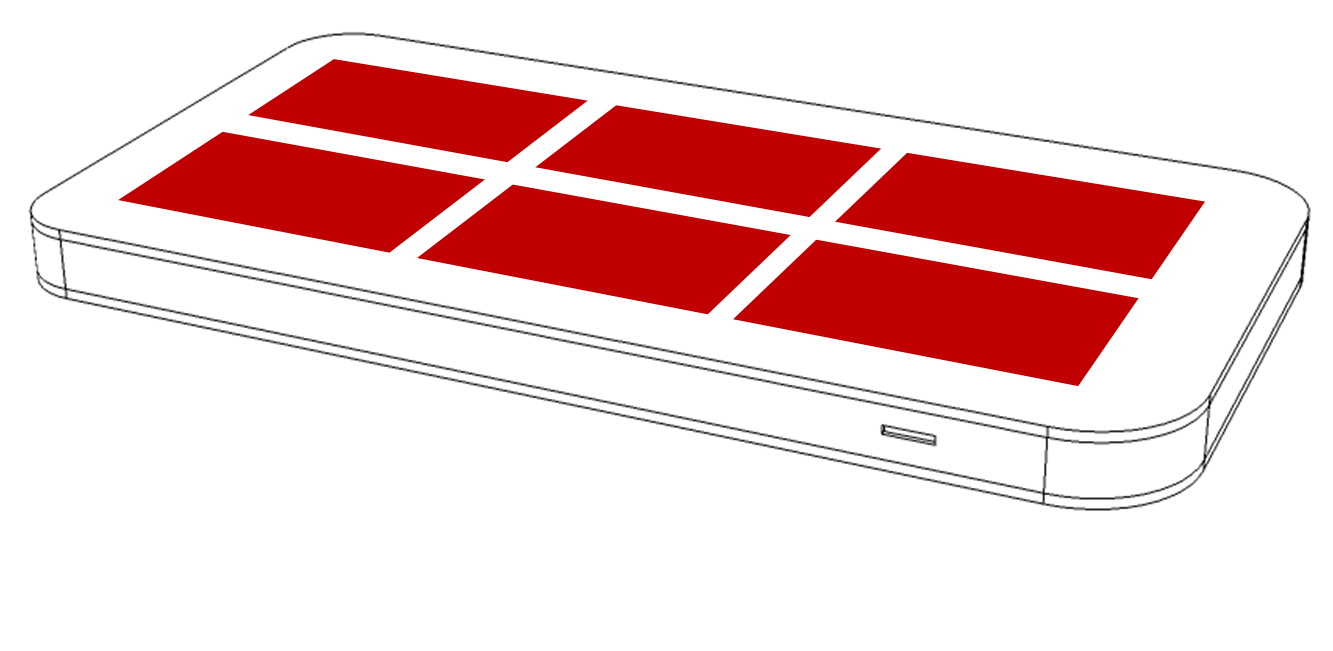
\includegraphics[width=0.6\textwidth]{images/magicbox}
\caption{MagicBox sketch - six electrodes uniformly distributed below surface}
\label{fig:magicbox_sketch}
\end{figure}
%Figure 28 MagicBox sketch - six electrodes uniformly distributed below surface
The so-called MagicBox was my first attempt to create an interaction device based on capacitive proximity sensing. For this prototype I collaborated with colleagues Pascal Hamisu, Tim Dutz and Felix Kamieth, as well as student Sebastian Jeckel. It is using an array of six individual wireless capacitive sensors that communicate to a central station \cite{Braun2011MultiInputDevice}. The system was later extended to support Machine Learning based gesture recognition adapted from mouse gestures \cite{braun2013capacitive}. The electrodes are using a large surface area and are made of aluminum foil. A sketch is shown in Figure \ref{fig:magicbox_sketch}. The system is able to track the position of a single hand in three dimensions up to a distance of approximately $20cm$. It uses different methods to infer gestures from the hand movement. 
It is designed to be a generic interaction device that can potentially be hidden below non-conductive surfaces. As it can be used without touching, it is also applicable in sterile environments. A suite of demonstration applications has been created that showcase typical scenarios for the MagicBox. This includes multimedia applications, like image viewer and media player but also a 3D object viewer intended as demonstrator for potential medical applications, allowing a surgeon to check MRT or CT images in a sterile environment without touching any surface.

\subsubsection{Evaluation}
\begin{figure}[ht]
\centering
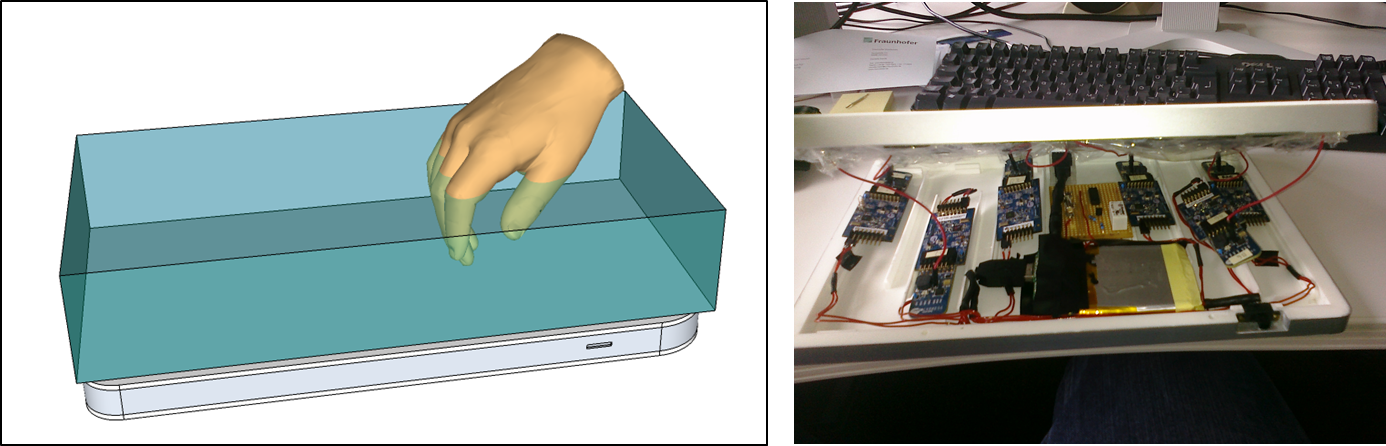
\includegraphics[width=0.8\textwidth]{images/magicbox_proto}
\caption{MagicBox conceptual rendering (left) and detail view of electronics (right) \cite{Braun2011MultiInputDevice}}
\label{fig:magicbox_proto}
\end{figure}

The MagicBox prototype is based on the Cypress First Touch starter kit \cite{cypressfirst} and combines six capaci-tive sensors communicating wirelessly to a single base station. They are put into a casing together with a USB-rechargeable power supply. A conceptual rendering showing the interaction area and a detail view of the prototype electronics are shown in Figure \ref{fig:magicbox_proto}.

\begin{figure}[ht]
\centering
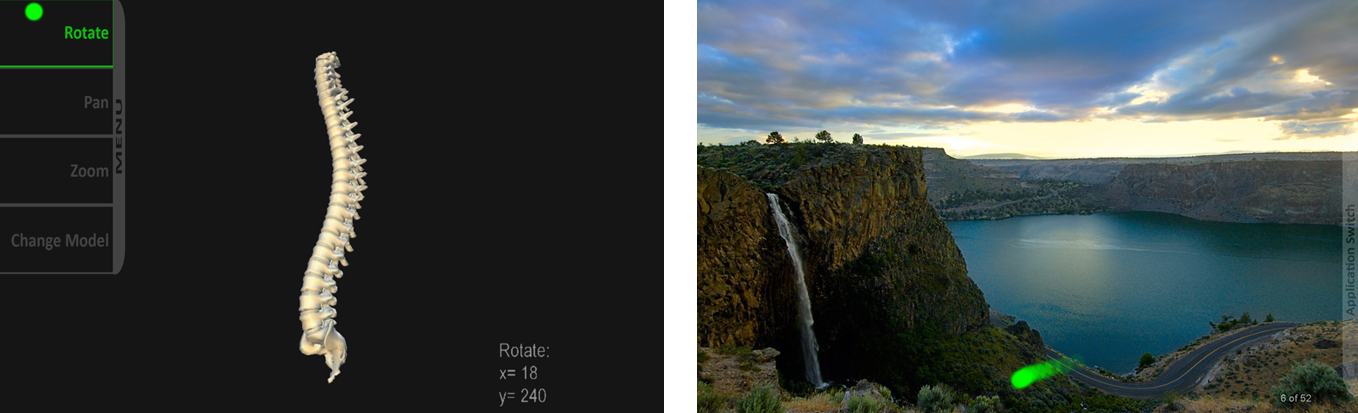
\includegraphics[width=0.8\textwidth]{images/magicbox_eval}
\caption{MagicBox demonstration application - 3D object viewer (left) and image viewer (right) \cite{Braun2011MultiInputDevice}}
\label{fig:magicbox_eval}
\end{figure}

The different iterations of the MagicBox have been evaluated in conjunction with various demonstration applications. A usability study with 18 persons led to general approval of the system \cite{Braun2011MultiInputDevice}. Two of the applications used in this study are shown in Figure \ref{fig:magicbox_eval}. On the left, there is a 3D object viewer that has to be controlled by a combination of menu and direct manipulation of the screen content. On the right side there is an image viewer that was controlled by gesture to trigger the next/previous images or perform zooming operations. The most common positive remarks gathered in this study can be roughly put into three groups:
\begin{itemize}
\item{The device very intuitive to use}
\item{The idea of interacting this way is novel and interesting}
\item{It is easy to control applications with those gestures}
\end{itemize}
Likewise we identified three main groups for negative comments about the prototype:
\begin{itemize}
\item{The device is not very precise}
\item{The interaction speed is slow}
\item{It can be tiring for the arm}
\end{itemize}
Later iterations have been trying to improve some of the weaknesses presented above, e.g. by using a more sophisticated gesture recognition system and faster sensor refresh rates. Accordingly, there were fewer complaints about interaction speed and precision \cite{braun2013capacitive}. However, the final complaint about the device being tiring for the arm, requires a different approach, that we are investigating in the next prototype to be presented in this section.

\begin{figure}[ht]
\centering
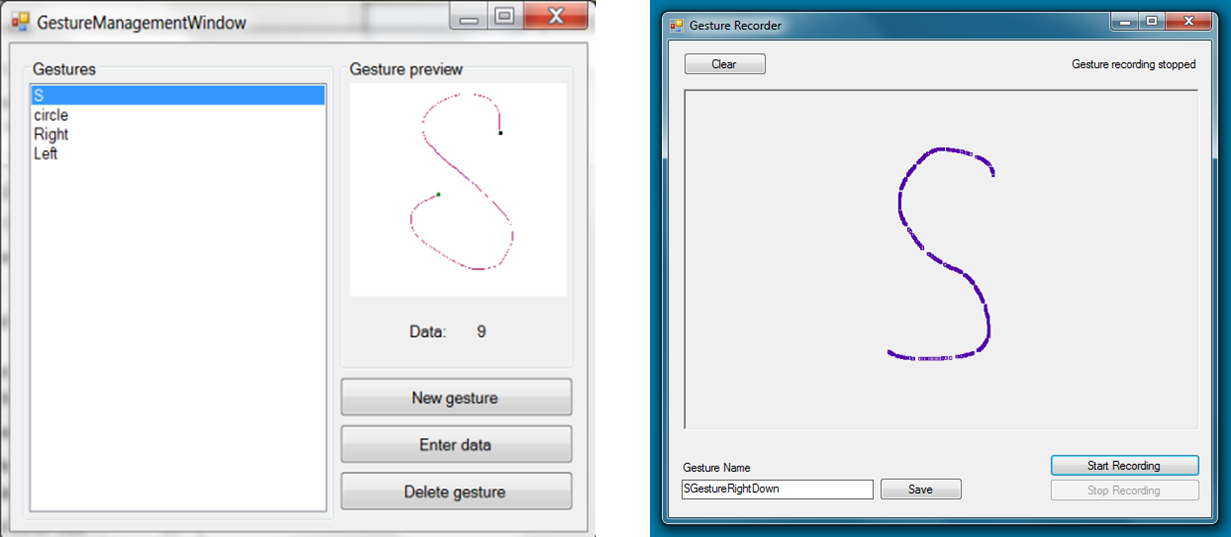
\includegraphics[width=0.7\textwidth]{images/magicbox_data_gest}
\caption{Gesture overview module (left) and gesture recorder (right) \cite{braun2013capacitive}}
\label{fig:magicbox_data_gest}
\end{figure}

The overall method is similar to mouse gesture recognition, albeit adapted for three dimensional locations. The developed system allows defining an arbitrary set of potential gestures and adding training data to each, as explained in section \ref{ch:proc_sparse}. The key aspect of gestures by example – providing examples - is realized in a debug application. It provides a simple way to record exemplary movements and associate them to gesture sets. The main screens realizing this functionality are shown in Figure \ref{fig:magicbox_data_gest}. On the left side we can see the management screen that allows adding and deleting gestures, as well as a preview that is an average of the sample data associated to this gesture. The process of entering data is shown on the right side, where several samples can be recorded and associated to the selected gesture. The user then can decide, whether the current movement should be stored or discarded.
